\documentclass[pscyr,titlepage,chapters]{hedreport}
\usepackage[russian]{babel}
\usepackage[utf8]{inputenc}
\usepackage{graphicx}
\usepackage{multirow}
\graphicspath{{images/}}

\usepackage{color}
\usepackage[colorlinks,linkcolor=black,citecolor=black]{hyperref}

\usepackage{setspace}

\faculty{Факультет экономики и управления}
\department{истории, культуры и социологии}
\type{Семестровая работа}
\subject{дисциплине <<Культурология>>}
\topic{Языческая символика как система мировосприятия древних славян}
\student[f]{студентка группы Ф-469\\Слоква В. И.}
\teacher[f]{ст. преп.\\Соловьева А. В.}

\begin{document}
  \maketitle
  \onehalfspacing
  \tableofcontents

  \chapter*{Введение}
  \addcontentsline{toc}{chapter}{Введение}

  Славянское язычество~-- это стройная система взглядов, которая пронизывала
  жизнь традиционного славянского общества, решая возникающие мировоззренческие
  вопросы, определяя коллективные приоритеты и вытекающие из них ценностные и
  деятельностные установки поведения людей.

  Жизнь древних славян была неотрывно связана с их верой. Данная связь ярко
  выражалась в различных символах, оберегах и обрядах.  Цель данной работы~--
  анализ славянского языческого миропонимания.

  \chapter{Роль символов в язычестве}

  Огромное значение в Вере Исконной, как любят называть язычество современные
  последователи древних волхвов, имеет символ, именно он, зачастую, несет в себе
  основную смысловую нагрузку в магическом и жреческом искусстве. Ведь символ~--
  это не просто значок или украшение на посохе волхва, обрядовой посуде, кумире
  или иной вещи, а совокупность сакральных смыслов, магических эффектов,
  многотысячелетних трудов древних гениев, формировавших сей знак.

  Символ применяется для воздействий на мир, преобразования его. Многие символы
  являются оберегами, <<отвращающими>> темные силы хаоса, способные причинить
  вред от носителя сего оберега, многие способны стереть грань между мирами,
  позволяющие, например, шаману, совершить путешествие в темный мир (Навь) или
  светлый (Правь), некоторые являются прямым обращением к богам, тем или иным
  силам природы.

  Славяне почитали богов жизни и смерти, плодородия и растительного царства,
  небесных светил и огня, неба и войны; олицетворялись не только солнце или
  вода, но и многочисленные домовые духи и т.~д.~-- поклонение и преклонение
  выражалось в принесении кровных и бескровных жертв. Славянские боги обитали
  на небесах; духи природы жили рядом с человеком: в доме, в поле, в лесах и
  реках. Славянские языческие боги олицетворяли силы природы: Перун~-- гром и
  молния, Род~-- род, Велес~-- мир животных и потусторонний мир и т.~д.

  \chapter{Обереги}
  
  Язычество находит выражение в вещественном мире. Человек чувствовал себя
  бессильным перед природой и ее стихиями; пытаясь понять их суть, раскрыть
  механизм влияния на него природы, обезопасить себя от неуправляемой стихии, он
  составлял целый комплекс взаимодействия с этими силами. Славяне-язычники
  общались с миром на языке оберегов~-- предметов, украшений, узоров, которые
  люди носили с собой и защищали ими свое жилище.

  Наиболее древними обережными символами были узоры, связанные с тремя стихиями,
  которым поклонялись славяне: символы земли, воды, огня. Их призывали славяне к
  себе в охранители. Символы земли~-- засеянное поле (ромб, разделенный на
  четыре части с точками внутри каждой), знак плодородия (свастика). Символ
  воды~-- хляби небесные (волнистые линии). Символ огня~-- косой крест (огонь
  земной), громовный знак (шести- или восьмилучевая звезда). Кроме этих,
  основных знаков, языческая символика включает изображение солнца, радуги,
  фигур богини на вершине строения, подковы и многие другие.

  \begin{figure}[ht]
    \center
    \begin{tabular}{*{3}{c@{\hspace{1em}}}c}
      \multirow{3}{*}{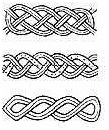
\includegraphics[height=9em]{sl_2_1}} &
        \multirow{2}{*}{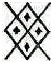
\includegraphics[height=4em]{sl_2_2}} &
        \multirow{3}{*}{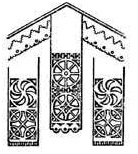
\includegraphics[height=9em]{sl_2_4}} &
        \multirow{8}{*}{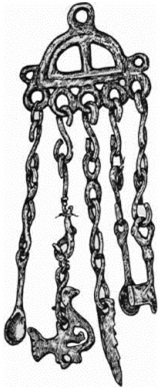
\includegraphics[height=24em]{sl_2_10}} \\[3em]
      & 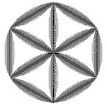
\includegraphics[height=4em]{sl_2_3} && \\
      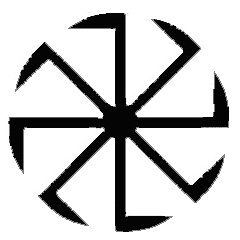
\includegraphics[height=6em]{sl_2_6} &
        \multicolumn{2}{c@{\hspace{1em}}}{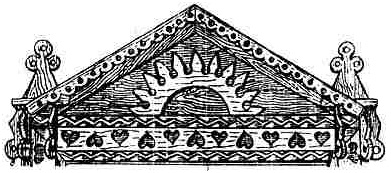
\includegraphics[height=6em]{sl_2_5}}
        & \\
      \multicolumn{2}{c@{\hspace{1em}}}{
        \multirow{3}{*}{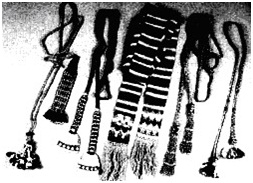
\includegraphics[height=9em]{sl_2_9}}} &
        \multirow{2}{*}{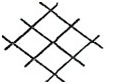
\includegraphics[height=4em]{sl_2_8}} & \\[3em]
      && 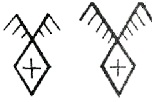
\includegraphics[height=4em]{sl_2_7} & \\
    \end{tabular}
    \caption{Примеры оберегов, орнаментов и символов}
  \end{figure}

  Языческие символы славяне размещают на <<уязвимых>> участках жилища и двора.
  Заклинательным орнаментом они закрывают все проемы, через которые нечистая
  сила может проникнуть к человеку: ворота, двери, окна, застрехи. Символ
  солнца, размещаемый в проемах, должен охранять жилище от ночной нечисти.
  Солярные знаки находим также на крыше дома~-- в виде конька, под крышей~-- в
  виде реального изображения солнца или его символа, на фасаде, на наличниках
  окон. На фасаде дома славяне изображают небо и ход солнца~-- утром, в полдень
  и вечером. При этом на центральном полотенце обычно размещают громовой знак
  (круг, разделенный на шесть секторов)~-- символ Рода или Перуна, оберегавшим
  дом от попадания в него молнии. Рядом с символом солнца почти всегда славяне
  изображают знак земли или засеянного поля, обозначающий единство небесного и
  земного, явного. Мир яви символизируют и изображения птиц, растений, богинь,
  переплетающиеся с фантастическими существами. Русалки-берегини защищают дом от
  нави, упырей. Чаще всего эти изображения находятся на наличниках окон, у входа
  в дом. Изображения оберегающих мир в доме Лады (богиня веселья, благополучия и
  согласия в семье; богиня невест) или Мокоши располагаются также на резных
  наличниках (они изображаются с поднятыми вверх руками, словно просящими защиты
  у верховных богов, дающих небесную влагу и свет), а также на хозяйственных
  постройках (они изображаются с опущенными руками, словно обращаются к
  матери-сырой земле, дающей урожай).
 
  Славяне старались защитить дом не только снаружи, но и изнутри, поэтому
  обереги располагали на матице (здесь помещали только коловрат~-- знак рода),
  над дверьми (самый распространенный оберег~-- подкова), на печи, на предметах
  быта. Причудливым орнаментом старались покрыть все, через что нечистая сила
  могла навредить человеку \cite{2}.

  Особую магию и особый смысл у славян имеют обрядовые полотенца. Узоры на них
  представляют не что иное, как славянский календарь, который образно отражал
  семейно-родовые события или аграрно-ритуальные торжества, свойственные
  земледельческой культуре. На всех праздниках первым на полотенце выносили хлеб
  да соль. Соль~-- символ солнца, любви; хлеб~-- земля, милость; полотенце~--
  символ жизни человеческой, полоса судьбы, часть чистого космического
  пространства. Во время обручения руки жениха и невесты соединяли, обернув
  полотенцем, чтобы молодые жили в достатке; с тем же смыслом во время родов
  бабка принимала младенца на новое полотенце. Полотенца-обыденники ткали и
  расшивали несложным обережным орнаментом против мора, для испрашивания дождя
  и т.~п., причем, чтобы полотенце имело чудодейственную силу, с работой ткачиха
  должна была справиться за один световой день. На погребальном полотенце
  изображались символы души и погребального (жертвенного) костра. Последний знак
  перекликается с символом земли, но ромб, состоящий из трех пар пересекающихся
  линий, оставался внутри пустым. Погребальные полотенца и полотенца-обыденники
  после совершения обряда отдавали в храм, на поминовение души.

  В одежде магическим охранительным узором покрывались ворот, обшлага рукавов,
  подол, разрезы, пояса. Сама ткань считалась непроницаемой для злых духов, так
  как в ее изготовлении участвовали предметы, изобильно снабженные магическим
  орнаментом (прялки, ткацкий стан).

  Наиболее тесно с жизнью человека связывают славяне пояс и воротник. Считается,
  что именно через воротник в случае смерти душа покидает тело, поэтому он
  обязательно оберегается узором. Охранных знаков здесь было такое множество,
  что со временем ворот превратился в отдельную наплечную часть одежды~--
  <<ожерелье>>. Пояс, опоясывая человека, проходит через пуповину~-- центр
  человеческого существа, его жизненное начало, поэтому он также должен быть
  покрыт обильной обережной вышивкой.

  Наиболее частым обереговым узором на одежде являются ромбы с крючками~--
  символами жизни. Кроме ромбов, значение амулетов, несущих огонь, тепло, жизнь,
  имели  круги и свастики с <<усиками>>, направленными по ходу солнца. В рукав
  обязательно вшивалась кумачовая ластовица, так как красный цвет, по поверью,
  отражает дурную энергию и защищает здоровье хозяина.

  Кроме вышитых и вырезанных узоров, славяне использовали и заклинательные
  привески-амулеты. В отдельных погребениях археологи находят целые наборы
  амулетов, подвешенных на цепочках на общей основе. Так, в составе одного из
  них имеются две ложки, птица, челюсть хищника и ключ. Ложка~-- символ сытости,
  благосостояния и довольства, ключ~-- символ богатства и сохранности. Челюсть
  или зуб хищника служили для ограждения от зла, для привлечения удачи на охоте,
  увеличения силы и мастерства. С древнейших времен славяне верили, что со
  звериными амулетами к ним переходят самые лучшие качества убитого животного.
  Привески в виде птиц и животных связаны были с их животными свойствами.
  Уточка, например, являлась символом продолжения Рода, счастливой семьи. Иногда
  в составе наборов привесок-амулетов обнаруживают бубенчики, которые своим
  звоном отгоняли злых духов; костяные ножи, служившие защитой от злых духов.
  Очень часто при раскопках обнаруживают зооморфные привески~-- так называемые
  <<коньки>>. Конь~-- символ добра и счастья; его связь с культом солнца
  подчеркивается солярными знаками на фигурках. Привески в виде других животных
  распространены мало.

  Особо нужно остановиться на ювелирных украшениях славян, которые также имели
  сакральное значение. Мужских оберегов сравнительно немного. Это, как правило,
  миниатюрное изображение оружия~-- ножи, мечи, топоры; маленькие коньки,
  которые являлись оберегом в пути и служили символом бога Перуна. Также мужчины
  носили когти и клыки диких зверей, добытых на охоте. Считалось, что так
  охотнику передается сила убитого зверя, которая помогает в охоте, защищает в
  лесу.

  Наибольшая защита требовалась женщине~-- продолжательнице рода. Обязательным
  оберегом у женщин являлись подвески, которые крепились на цепочках и носились
  на поясе, как ожерелье или у плеча. Часто они были сделаны в виде коня или
  утко-коня, к ним также крепились бубенчики или утиные лапки~-- символ Рода как
  создателя земли. Еще одним обязательным элементом подвесок был семилучевой
  гребешок, который означал здоровье и должен был оберегать женщину от болезней
  и дурного глаза. Третий элемент подвески~-- ложечка символизирует сытость,
  достаток в доме; четвертый~-- ключ означает богатство. Также в подвесках
  встречаются маленькие ножи, серьги~-- символ урожая; изображение Чура~--
  охранителя домашнего очага. Встречается на подвесках и пестик от ступы~--
  символ мужского начала, плодовитость. Подвески~-- бляшки имели самый
  разнообразный характер, и могли носиться как женщинами, так и мужчинами в
  качестве нательного оберега. Как правило, бляшки имели солярную, земную и
  зооморфную символику: солнечный крест, означающий выбор человеком жизненного
  пути, восьмиконечный крест~-- символ Рода, ромбики~-- знаки земли, изображение
  птиц, зверей, свастики~-- все это являлось основными узорами орнамента
  подвесок. Женские подвески изготавливались из бронзы или иного желтого,
  солнечного металла.

  Одним из главных женских украшений является головной убор~-- венчик у девушек,
  кика или кокошник у замужних женщин. Венок~-- круг-оберег, сохраняющий добрые,
  светлые мысли. Кика символизировала собой рог тура или матери-оленихи, она
  должна была придавать женщине силу. Головной убор отделывался бисером,
  украшался нитями жемчуга~-- ряснами~-- и височными кольцами~-- колтами.
  Височные кольца напоминают гребешок петуха, или восходящее солнце. Поверхность
  их покрывается знаками, похожими на руны, а также знаками Мокоши \cite{6}.

  Ожерелья состояли из отдельных подвесок и лунниц. Лунница~-- исключительно
  женский оберег, так как луна всегда считалась женской планетой. Лунница
  оберегала от ночных духов и нави, просыпающихся при свете луны. Их
  изготавливали, как правило, из серебра или другого серебристого металла,
  символизирующего луну. Составными частями женского ожерелья являлись также
  бусины из стекла, кости, камни и бляшки-подвески. Иногда в качестве подвесок
  использовались монетки. На шее женщины иногда могло быть несколько ожерелий,
  состоящих из лунниц, бляшек и бусин. Количество украшений показывало статус
  женщины и, разумеется, имело оберегающий характер.

  Браслеты носились и мужчинами, и женщинами, они скрепляли рукава одежды и тем
  самым не только делали ее удобной в носке, но и оберегали от проникновения
  нечистой силы. Браслеты были стеклянные, костяные, из крученой проволоки, из
  полосок металла, створчатые. На браслетах изображались символы земли и солнца.
  Женские створчатые браслеты скрепляли на запястьях рукавов ритуальных
  русальных рубах; во время праздничных хороводов эти рукава распускались для
  ритуального танца.

  Неизменность языческой символики на протяжении многих столетий говорит о том,
  что славяне даже после принятия христианства долго сохраняли многие черты
  исконной религии, которые касались обыденной жизни человека. Постепенно мифы и
  значения символов стали забываться, однако осколки язычества дошли до наших
  дней в народных поверьях, обычаях и традициях \cite{3}.

  \chapter{Символы небесных светил в орнаменте Древней Руси}
 
  Обоготворение и почитание неба и небесных светил занимает огромное место в
  системе религиозных верований древности. Эти культы в той или иной степени
  свойственны всем без исключения земледельческим скотоводческим и охотничьим и
  племенам, занимающихся ловлей рыбы, конвергентно возникая на определенной
  стадии общественно-экономического развития.

  Небесные верования восточных славян, среди которых выделяется аграрный культ
  солнца, воплотились в символических знаках, своеобразных идеограммах, которые
  занимают видное место среди других мотивов древнерусской орнаментики.

  Все эти символы оказались настолько устойчивыми, что в качестве декоративных
  элементов сохранились в народных узорах (резьба по дереву, вышивка) до наших
  дней, что было отмечено многими исследователями.

  На рис.~\ref{pic42} дан генеалогический ряд этих знаков по степени усложнения
  форм, хотя как простые, так и сложные формы зачастую синхронны.
 
  \begin{figure}[ht]
    \center
    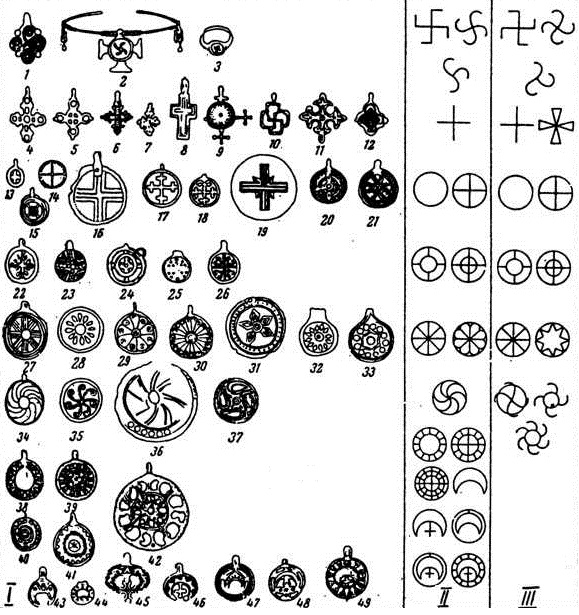
\includegraphics[width=.8\textwidth]{sl_3_1}
    \caption{Солнечная символика в славянских украшениях по Ж.~Дешелетту:\\
      I~-- общий вид украшений; II~-- схема орнамента на них; III~-- знаки,
      употреблявшиеся как солнечные символы в бронзовом и железном веке}    
    \label{pic42}
  \end{figure}

  Крест~-- древний магический символ, существовавший задолго до христианства у
  самых различных народов. Первоначально форма креста имитировала древнейшее
  орудие для добывания огня, поэтому он стал универсальной религиозной эмблемой
  огня, а затем солнца как огня небесного. Как и огонь, солнце умирает и
  возрождается в процессе движения по небу. Крест как эмблема солнечного
  божества становится языческим очистительным символом воскресения и бессмертия
  задолго до христианства. У языческих славян крест был также символом огня.
  Огонь, по языческим поверьям, был очистительной, целебной стихией, способной
  отпугивать нечистую силу. Поэтому графический символ этой стихии~-- крест,
  играет аналогичную роль. Его широкое распространение в народной среде говорит
  о древних корнях этого символа. В пережиточных народных обычаях связь огня с
  фигурой креста выступает достаточно четко. Например, на Украине в Великий
  Четверг приносили из церкви страстную свечу, огнем которой выжигали кресты на
  волоках. Кресты ставили в избах, над окнами, воротами, дверями, на разных
  местах около дорог, по краям улиц, на перекрестках, на пожнях, на высоких
  берегах, над могилами. Крест носят на шее, помещают на свадебном пироге и
  т.~п. В некоторые праздничные дни (например, в Коляды) был широко
  распространен обычай чертить мелом кресты не только на домах и хозяйственных
  постройках, но на всех земледельческих орудиях, на мебели, посуде и т.~д. Этот
  обряд совершался для изгнания злых духов. Иногда хозяин, рисуя кресты, держал
  в руках блин, которые некоторые исследователи считают символом солнца.

  В древнерусских курганных древностях \emph{X}--\emph{XIII}~вв. Повсеместно
  распространены подвески-крестики разнообразных форм (рис.~\ref{pic42}: 4-12),
  многие из которых не имеют никакого отношения к христианству.

  Подвески-крестики \emph{XI}~в. найдены в земле радимичей в костромских
  курганах \emph{XI}--\emph{XII}~вв. где язычество было еще в то время очень
  сильно. Иногда они встречаются на одной цепочке с другими амулетами (коньками,
  ложечками, зубами зверя).

  Крест являлся одновременно и символом молнии. В древности были широко
  распространены представления о небесном происхождении земного огня. Огонь
  считался посланием небес, даром неба, низведенным на землю. В свою очередь
  небесные светила считались средоточием небесного огня. У татранских словаков
  существовало предание о том, что огонь породил и солнце, и месяц, и звезды. У
  других славян существовали подобные.

  Связь небесного (солнце) и земного огня явственно выступает в праздничной
  народной обрядности. Так, Коляды~-- праздник зимнего солнца~-- повсюду
  сопровождались возжением огней. Это было или бревно-бадняк, с особыми обрядами
  сжигавшееся в печи, или огонь свечей. Первоначально эти огни зажигались,
  по-видимому, с магическими целями заклинания солнца. Они являются необходимой
  принадлежностью и праздника Ивана Купалы в честь летнего солнца. Иногда эти
  огни в народе прямо назывались огнями неба, и их получали посредством вращения
  колеса (символа солнца) вокруг оси. Живой огонь, добытый таким путем, считался
  священным, обеззараживающим, способным давать обильный урожай именно благодаря
  тому, что был призван подражать теплу и свету солнца. Вследствие связи
  почитания солнца и огня они обозначались единым символом~-- фигурой креста. В
  то же время крестообразные фигуры заключали в себе и более сложную символику.

  Крест~-- фигура, образованная четырьмя лучами. Число 4 у многих народов, в том
  числе и у славян, было магическим, священным (понятие о четырех стихиях,
  четыре времени года, четыре стороны света). Два последних значения тесно
  связывали число 4 с культом солнца. Так, бог Святовит имел четыре головы,
  Збручский идол имеет четыре лика, обрамленные к четырем сторонам горизонта.
  Святилище, открытое В.~В.~Хвойкой в Киеве, имело четыре выступа,
  ориентированные по сторонам света. Подобно этому, на шаманских бубнах у саамов
  солнце изображалось кружком с четырьмя лучами
  \( \big(+\hspace{-11.6pt}\circ \hspace{4pt}\big) \), 
  которые называются четырьмя вожжами солнца. Это обозначало, что власть солнца
  распространяется на всю землю.

  Можно предположить, что у языческих славян крест, являясь священным символом
  солнца-огня, служил также амулетом, оберегавшим его владельца со всех четырех
  сторон. К кругу тождественных представлений, по-видимому, относятся подвески,
  где орнаментируемая плоскость делится на четыре части с заполнением узором,
  каждой, из них (рис.~\ref{pic42}: 25, 26). К схеме креста восходит и так
  называемая четырехчастная, известная по орнаменту дробниц поясных наборов
  \emph{Х}--\emph{XI}~вв.

  В народном искусстве до сих пор можно найти отголоски древних представлений,
  связанных с описанными четырьмя элементами.

  Свастика~-- повсеместно распространенный древний символ огня и солнца. По
  происхождению и содержанию близка кресту. По внешнему виду отличается от него
  отростками, оканчивающими каждый луч, которые первоначально символизировали
  вращательное движение древнего приспособления для добывания огня, а затем,
  когда свастика стала символом солнца, обозначали его движение по небу.

  В качестве солярных эмблем известны прямолинейная и криволинейная свастика.
  Древней Руси известны оба вида свастики, однако этот знак и его разновидности
  встречаются сравнительно редко, обычно в виде единичных изображений
  (рис.~\ref{pic42}: 1-3). В народной вышивке, на писанках свастика сохранялась
  до недавнего времени.

  Из свастики посредством уничтожения одной ветви образуется триквестр~-- знак
  огня, домашнего очага, три изогнутые отростка которого напоминают трепетные
  языки пламени. Триквестр присутствует в составе символической композиции на
  серебряном браслете \emph{ХII}~в. из Чернигова.

  Форма круга издавна связывалась с постоянно наблюдаемой формой солнечного
  диска. В восточнославянских курганных древностях, известны круглые подвески
  без орнамента, возможно имитирующие солнце.

  Крест и круг два основных элемента, из которых посредством сочетания и
  видоизменений образуются остальные солнечные символы. Крест в круге
  (рис.~\ref{pic42}: 13-24). Этот древний знак, возможно вначале воплощал идею о
  неразрывной связи небесного (солнце) и земного огня, затем~-- повсеместно
  распространенная идеограмма солнца. Иногда такой крест видоизменяется в
  четырехлепестковый цветок (рис.~\ref{pic42}: 20). Подобные формы
  непосредственно переходят в розетку.

  Колесо~-- один из самых употребительных солярных символов (рис.~\ref{pic42}: 27).
  Уже не четыре, а много лучей (спиц) исходит из одной точки. Уподобление колеса
  солнцу было повсеместно распространено в Восточной и Западной Европе. Эта
  ассоциация с огненным колесом основана на том, что, по древним представлениям,
  солнце вертится, катится по небу.
  Купальский огонь, символизирующий солнце, иногда зажигался посредством
  вращения колеса. Колесо, облитое дегтем, зажигалось на масленицу, когда оно
  символизировало возрождающееся после зимней спячки солнце, и на Ивана Купалу,
  когда солнце поворачивает на зиму.
  
  Розетка (рис.~\ref{pic42}: 28-30) уже в древнейших культурах Востока была
  эмблемой солнечных богов. Фигура розетки оказалась наиболее устойчивой и в
  декоративной народной резьбе по дереву является одним из основных элементов
  узора. По своему начертанию она близка к цветку (рис.~\ref{pic42}: 31). В
  розетке как бы воплотилась идея о связи животворящих солнечных лучей и
  обильного произрастания цветов и трав на земле.

  Круг с вращающимся расчленением (так называемое сегнерово колесо) является
  графическим изображением вращающегося колеса-солнца (рис.~\ref{pic42}: 34-37).
  Загнутые в одном направлении спицы символизируют движение. Фигура близка
  криволинейной свастике. Это форма обычна в современной резьбе по дереву.

  В восточнославянских древностях \emph{Х}--\emph{XIII}~вв. повсеместно
  распространены подвески-лунницы, в которых нашло отражение древнее почитание
  луны. Некоторые из них покрыты растительным орнаментом (рис.~\ref{pic42}: 45).
  В связи с этим интересно вспомнить народные поверья, по которым луна влияет на
  рост растений и развитие цветов. Лунницам приписывались священные свойства.

  Вся композиция воспринимается как единый солярно-лунарный символ. Вместе с тем
  она могла иметь более широкий смысл, нести двоякую символику. В языческих
  религиях почитание солнца и месяца как божеств~-- покровителей брака,
  представляет очень распространенное явление. Месяц обычно является началом
  мужским, женихом, солнце~-- невестой. Эти небесные светила являются
  божественной брачной парой, брак которых служит прототипом человеческих
  браков. Как божествам, живущим в браке, земные браки отдавались под
  покровительство солнца и месяца. В славянской народной поэзии женский облик
  солнца обычнее, чем мужской, причем солнце и месяц также часто являются
  супружеской парой. В белорусской свадебной поэзии месяц неизменно мужское
  начало, солнце~-- женское. В славянских колядных песнях хозяин сравнивается с
  месяцем, а его жена~-- с солнышком. В свадебном хлебе также иногда заключается
  мысль о браке солнца и месяца и самому хлебу придается форма солнца или
  месяца, а иногда он представляет все небесное семейство: в углублении каравая
  помещают сделанные из теста изображения солнца и луны.

  Таким образом, композиция из луны с крестом могла обозначать неразрывность,
  единство мужского и женского начал, быть символом супружества. Этот древний
  языческий символ дожил до последнего времени в крестах
  с полумесяцем под ним на куполах русских церквей. Позднее такая композиции
  воспринималась как символ победы христианства над магометанством. Дальнейшее
  усложнение этого мотива представляют собой подвески, где луна с крестом
  заключается в ободок (рис.~\ref{pic42}: 48). Особенно интересна подвеска
  (рис.~\ref{pic42}: 49), воплощающая целый комплекс космических верований
  древних славян, соединяющая в одном символе все небесные элементы. Она
  представляет собой крест внутри лунницы, от которой расходятся 12~лучей. Вся
  композиция помещена в круглый ободок. Семантика луны с крестом выявлена выше.
  Что же означают остальные элементы композиции? Очень часто количество
  повторяющихся элементов в орнаменте рассматриваемых подвесок равно~12
  (12~лепестков розетки, 12~лучей, шариков, идущих по кругу и т.д.)~--
  рис.~\ref{pic42}: 28, 32, 33, 38, 40, 42, 49. Священное число~12 у славян было
  связано с небесными верованиями. Оно постоянно фигурирует в мифологических
  сказаниях, где представления о небе и солнце выступают в аллегорической форме.
  У всех славян сохранились предания о царе-солнце и его золотых чертогах; у
  него~12 сыновей и 12~солнечных. У солнца~12 царств, каждым из которых владеет
  один из его сыновей, которые живут в звездах.

  Того же происхождения загадка: рассыпался горох на двенадцать лугов~-- звезды.
  Число~12 выступает иногда в обрядовых действиях, связанных с почитанием
  солнца. В некоторых местностях
  России на масленицу на санях, запряженных 12 лошадьми, возили наряженного
  мужика, который сидел на колесе наверху столба, поставленного посередине
  саней. Во всех этих преданиях и обрядах нашло отражение деление года на
  12~месяцев. Рассматриваемая композиция представляет собой символическое
  изображение солнца с его 12~чертогами (месяцами) и луны (т.~е. всего небесного
  семейства), заключенных в круглый ободок, вероятно, символизирующий небо,
  небесный круг, по которому совершают свой путь солнце и луна. Иногда из этой
  композиции выпадают отдельные элементы; например, у подвески, изображенной на
  рис.~\ref{pic42}: 38, сохранились лишь два ободка с 12~маленькими лучами между
  ними. Иногда во внутренний ободок вписывается крест (рис.~\ref{pic42}:~39).
  На рис.~\ref{pic42}:~40, 41 представлены три концентрических ободка с
  12~лучами между ними и с крестом внутри. Это как бы две небесные сферы с
  солнцем в центре. Возможно, подобные подвески отражали более сложные
  представления о небе. Так, в ряде народных сказаний небесный круг делится на
  две части: летнюю и зимнюю. Возможно, средневековые схоластические сказания о
  многочисленности небес имели древнюю языческую основу, что и нашло отражение в
  данной композиции.

  Таковы основные небесные символы, известные в древней Руси. Их магические
  функции закономерны, так как солнце и луна представлялись добрыми божествами
  карателями всякой нечистой силы и зла; их появление приносило жизнь, здоровье,
  благополучие. Эти свойства были перенесены на условные изображения этих
  светил, игравшие роль чудесных оберегов \cite{1}.

  \chapter{Символика Природы, Земли и плодородия}

  Мать-земля, Матушка-природа. Все знают такие словосочетания, но мало кто
  задумывался, почему так говорят. А ведь это выражение пришло к нам из
  Язычества. Нет ничего удивительного в том, что наш предок, язычник, мог
  назвать землю матерью~-- она, подательница всех благ. Она и кормит и поит, и
  одевает и греет. Земля в союзе с небом (в народной мифологии~-- они супруги)
  дает нам тот мир, в котором мы живем. Естественно, Земля не могла не
  отразиться в мифологии и народных преданиях. Богиня Земли, плодородия и
  судьбы~-- Макошь. Ее имя образовано из двух корней~-- <<Ма>> (Мать) и <<Кошь>>
  (кошелек, хранилище богатства). Такая расшифровка дает четкое представление о
  том, как относились наши предки к Макоши и самой Земле. Земля ассоциируется с
  женским началом~-- во-первых, Земля способна родить жизнь, во-вторых, ее
  сестры, Доля и Недоля прядут нити судьбы (Доля прядет счастливую судьбу,
  Недоля~-- несчастную), ведь нить~-- символ жизни. У Доли нить мягкая, ровная,
  у Недоли~-- хлипкая, тонкая, как и судьба человека. Когда нить обрывается,
  человек погибает. Неприменный атрибут Макоши~-- рог изобилия, еще раз
  говорящий о ее значимости для людей и отношении к земле.

  \begin{figure}[ht]
    \center
    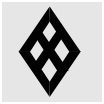
\includegraphics{sl_5_1} \hspace{1em}
    
\includegraphics{sl_5_2} \hspace{1em}
    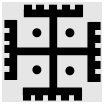
\includegraphics{sl_5_3} \hspace{1em}
    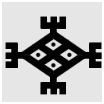
\includegraphics{sl_5_4}
    \caption{Символы незасеянного и засеянного полей}
    \label{pic-fields}
  \end{figure}

  Символика плодородия является одной из важнейших в культуре славян.
  Она представлена очень характерным
  узором~-- ромбом (или квадратом), разделенным внутри еще на четыре ромба.
  Это~-- поле. Маленькие ромбики~-- лунки для семян. Если в
  маленьких ромбиках изображаются точки, это значит, что поле засеяно~-- это
  символ плодородия. Если маленькие ромбики пусты, значит поле не засеяно
  (рис. \ref{pic-fields}). Символы эти имеют соответственное магическое
  значение. Возможны бесчисленные
  вариации с ромбами, квадратами и точками. В целом, ромб (квадрат) с точкой
  посередине~-- это то, что может родить, то, что является источником
  благополучия и изобилия.

  Пустой ромб~-- то же, но не могущее (не оплодотворенное) родить.
 
  Символы же природы очень многочисленны и многогранны. Нет такого символа,
  который бы означал саму природу. Зато ей посвящено довольно много магических
  знаков. Это прежде всего, природа волшебная. Поэтому, начну с символов
  Мирового Древа (рис.~\ref{pic-world_tree}). Мировое Древо
  (у скандинавов~-- ясень Иггдасиль)~-- <<Ось мира>>, оно держит на себе все
  миры. В кроне расположился мир Прави. У ствола~-- Явь, в корнях, там где
  ютится Мировой Змей Юша~-- Навь. Шаман, будучи в трансе, может совершить
  путешествие по этим мирам. Отголосок древнего
  мифа о Мировом Древе мы видим в сказке про волшебный боб, там старик
  выращивает волшебную бобовую лозу до самого неба и забирается по ней на
  облака.

  Особо известен такой символ, как цветок папоротника
  (рис.~\ref{pic-fire_flower}), с которым связана легенда~-- папоротник в ночь
  на Купалу выпускает красивейший цветок-огнецвет. И цветет он только одну ночь,
  а потом бесследно пропадает. Тот, кто найдет этот цветок, станет мудрым и
  сильным.

  Не волшебная природа тоже нашла отражение в символах. Например, лес
  (рис.~\ref{pic-forest}) изображался как несколько схематически нарисованных
  деревьев. Причем, обратим внимание, что при разложении такого дерева, мы
  получим из <<елочки>> несколько Футаркских рун Тейваз (\emph{Teiwaz}), руну
  воинов, атакующих сил или руны Ансуз (\emph{Ansuz}), что значит <<Бог>>~-- эта
  руна связана с Богами, а также с путешествием по Мировому Древу
  (рис.~\ref{pic-world_tree}) \cite{5}. Воспользовавшись вендскими рунами, елка
  предстанет перед нами как сочетание рун <<Алатырь>>, <<Нужда>>, <<Леля>>,
  <<Треба>>. Ясно, что <<Елка>>, а скорее, Сосна~-- дерево веры и магии. Не
  елка, а сосна потому, что~-- ель, дерево темное. В доказательство~-- Русская
  пословица: <<в березовом лесу веселиться, в сосновом~-- молиться, а в
  еловом~-- повеситься>>. Однако ель здесь возможна как темная, навская сторона
  веры. Теперь рассмотрим <<елку наоборот>>, чьи ветки направлены вверх.
  Расчленим ее тоже на руны. Перед нами футаркские~-- Феху (\emph{Fehu})~--
  владение (зачастую, духовное) и Альгиз (\emph{Algiz})~-- пассивная защита. В
  вендских~-- <<Мир>>, <<Крада>> (жертвенный огонь), Берегиня (женская руна,
  руна Макоши) и <<Есть>> (естество, жизнь, движение). Теперь понятен сакральный
  смысл с виду примитивных <<елочек>>. Тогда как <<Сосна>> направлена к
  божественному аспекту веры, <<перевернутая сосна>>~-- аспект более
  человеческий, мирской~-- богослужения, традиции, жертвоприношение, продолжение
  рода.

  Также и животный мир получил отражение в символах. Знаки унаследовали свойства
  животных. Особый же смысл имеют знаки, обозначающие птиц, ибо птица~-- существо
  для древних загадочное, магическое. Многие светлые боги могут обращаться в
  птицу. Перун~-- в орла или ворона, Волх~-- в Финиста-Сокола. Интересен общий
  для всех птиц знак~-- <<птица клевучая>>. Она символизирует небо, наследие
  светлых богов, в какой-то степени самих богов.

  Существуют также свастикоподобные символы <<птицы>>, например, знак ворона
  (рис.~\ref{pic-bird}). Даже на русском гербе~-- орле с распростертыми
  крыльями~-- можно увидеть очертания свастики.

  \begin{figure}[ht]
    \center
    
\includegraphics{sl_5_5} \hspace{1em}
    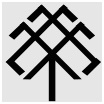
\includegraphics{sl_5_6} \hspace{1em}
    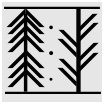
\includegraphics{sl_5_7} \hspace{1em}
    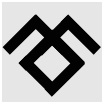
\includegraphics{sl_5_8} \\
    \parbox{6em}{\caption{Мировое древо}\label{pic-world_tree}} \hspace{1ex}
    \parbox{6em}{\caption{Огнецвет}\label{pic-fire_flower}} \hspace{1ex}
    \parbox{6em}{\caption{Лес}\label{pic-forest}} \hspace{1ex}
    \parbox{6em}{\caption{Ворон}\label{pic-bird}}
  \end{figure}

  Можно также посмотреть на русские вышивки~-- на них тоже часто фигурируют
  птицы. Но птицы эти уже не явские, а волшебные~-- известные всем по сказкам и
  песням Сирин, Алконост, Гамаюн. Птицы эти сидят на ветвях Мирового древа и
  поют свои песни. Изображаются они не так схематично, как другие, но их
  изображения несут в основном, эстетических характер~-- для магии и
  богослужения их не применяют. Возможно эта их отрешенность от волшебства,
  позволила этим символам дожить до наших времен в виде вышивок, резных и
  глиняных изделий.

  \chapter{Символика Воды}
  
  Вода, одна из творческих стихий, очень интересна с языческой точки зрения, у
  нее очень много сакральных аспектов, что не может не отражаться на ее
  символике. Во-первых, вода для язычника, это то, что дает жизнь всему
  живому. А ведь именно при помощи животворящей небесной воды зеленеют травы и
  леса весной, именно благодаря ней урожай не засыхает в поле, а цветет,
  плодоносит и колосится. Древние наши пращуры вполне это осознавали.
  Именно из воды родилась земля, принесенная в клюве Мировой Уточки по
  одному из древних Русских мифов. Также Вода несет в себе сакральный смысл
  очищения. Язычник, моющийся в бане смывает с себя не только грязь физическую,
  но и грязь духовную~-- оболочку порока, тьмы, ненависти. Получается ритуал,
  ведь совершается священнодействие перерождения, обновления человека~-- подобно
  обновлению кожи и тела человека в бане, обновляется душа, его аура. Омовение
  совершалось перед важными делами~-- жрец обязательно должен помыться в бане,
  чтобы совершить обряд, человек должен помыться, например, перед свадьбой~--
  прежде всего не для красоты, а для того, чтобы ритуалу не помешали темные
  силы. Воин же всегда мылся перед битвой, и после битвы, дабы на сражение не
  повлияли все те же силы. И третий по счету, но далеко не последний аспект
  значения воды для язычника~-- это ее течение. Все знают пословицу, что два
  раза в одну и ту же реку не войти. Многие ее не понимают~-- для них река эта
  синяя линия на карте. Для язычника же река~-- это поток воды~-- вода утекла и
  река другая. То есть течение воды это своего рода показатель времени. Недаром
  говорят~-- <<сколько воды утекло с тех пор>>, имея в виду, что прошло много
  времени. Так что текучая речная вода, это и сакральное сравнение с временем -
  вода неизбежно утекает, как и утекают дни, годы, века.

  Соответственно, символы воды имеют различные значения.

  Животворящая вода~-- вода небесная вода, или как любят ее называть, <<хляби
  небесные>>. Именно
  благодаря этой воде, растения питаются, набираются сил~-- трава становится
  зеленой и сочной, рожь колосится, репа вырастает как в известной сказке.
  Дождь, поливая поле, дает жизненную силу растениям, наполняет их соками. Также
  с небесной водой связано представление о роге изобилия. Дело в том, что сочные
  травы играли стратегическую роль в древности~-- скоту надо было где пастись, а
  если есть где пастись, значит есть в изобилии молоко и мясо. Если есть дожди,
  значит на поле будут колоситься хлеба и давать большие урожаи овощи на
  грядках, а значит в изобилии у нашего предка будут хлебобулочные изделия и
  большие запасы овощей на зиму. Иногда поэтому рог изобилия даже изображают как
  бы льющим воду.

  Совсем другая вода~-- речная, в отличие от дождевой, она в основе своей,
  пришла как раз из-под земли~-- из ключей, родников. Между прочим, родник
  считался священным местом~-- осквернить его было тоже, что осквернить капище.
  Ведь в роднике <<рождается>> вода~-- приходя из недр земли, она течет из
  родника тоненьким ручейком, ручеек соединяется с другим, эти соединяются с
  третьим~-- так получается могучая река. Некоторые родники обладали
  чудодейственными целительными свойствами. Поскольку ключевая и речная вода
  течет, ее изображают волнистыми горизонтальными полосами. Вода речная, в
  отличие от дождевой и наряду с нитью, может выступать как символ течения
  времени, жизни. Вода утекает вместе с навсегда ушедшими прошлое мгновениями.
  Вода~-- это не просто судьба, эта сила того, что
  ведет, то есть в воде есть сакральный символизм рока, того, от чего уйти
  нельзя. В старшем Футарке существует руна <<Лагуз>> (\emph{Laguz}), <<Вода>>.
  Ее значение как раз отображает суть текущей воды.

  В Традиции существуют также удивительные предания о волшебных реках, знакомыми
  по сказкам~-- это Ирийская молочная река, вытекающая
  из-под камня Алатыря (что на острове Буяне)~-- символизирует она не
  что-нибудь, а млечный путь. Молочная река~-- это поэтическое представление
  окраин нашей галактики. Млечным путем и молочной (Белой) рекой связано
  множество преданий, большинство~-- с рассказами о жизни после смерти. Однако в
  этих рассказах фигурирует еще одна река, Смородина, огненная река. Она
  разделяет Явский мир и <<великие просторы Нави>>. Стережет границы Нави
  знакомая многим, если не всем, Баба Яга (Буря Яга).

  С мифическими реками также связано представление о Калиновом Мосте. Калинов
  мост~-- понятие многогранное и очень сложное. Он связан с тонкими состояниями
  человеческой души~-- любовью, высокими чувствами. В поздние времена
  <<Встречаться с кем-то на Калиновом Мосту>>~-- значит любить. Однако, не все
  так радужно. На самом деле, на Калиновом Мосту проходит главная битва людской
  души между началом Прави и Нави~-- бой с самим собой (наша жизнь~-- вечная
  борьба).

  \chapter{Символика Огня}
  
  Огонь. Наверное, даже самый городской человек хоть раз в жизни смотрел на
  живой огонь, не из газовой плиты или зажигалки, а настоящий, который в печи
  или костре. Зрелище, завораживающее глаз и ум. Естественно, что у Язычника
  огонь вызывает те же чувства. Огонь для Язычника, это не просто химический
  процесс, это сакральное явление. С этим явлением напрямую связаны понятия об
  огне жертвенном (земной огонь, рис.~\ref{pic-earth_fire})~-- дым от
  жертвенного костра уносит в Ирий сущности жертв (сущности потому, что сложно
  сказать, что к примеру, у блина есть душа или нет, а вот сущность есть у
  любого предмета). Также существует огонь небесный (рис.~\ref{pic-sky_fire})~--
  огонь небесной кузни, кузни Сварога, Тора~-- одна из основных творческих сил.
  Проведем некоторые аналогии с Солнцем и плазмой и теорией большого взрыва и
  периодом формирования Земли, когда на ней происходили активные тектонические
  процессы, извержения вулканов. Уместно будет также вспомнить об огненном
  мече~-- символе справедливости и Прави, которым вооружены многие герои
  фэнтезийные и исторические персонажи даже в современных произведениях.

  \begin{figure}[ht]
    \center
    
\includegraphics{sl_7_1} \hspace{1em}
    
\includegraphics{sl_7_2} \hspace{1em}
    
\includegraphics{sl_7_3} \hspace{1em}
    
\includegraphics{sl_7_4} \hspace{1em}
    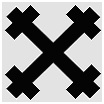
\includegraphics{sl_7_5} \\
    \parbox{12.5em}{\caption{Небесный огонь}\label{pic-sky_fire}} \hspace{1em}
    \parbox{20em}{\caption{Огонь земной}\label{pic-earth_fire}}
  \end{figure}

  Также существует огонь Нави, здесь приведу аналогии с христианскими
  культом, в котором грешников, пребывающих в аду жарят черти на кострах, у
  которых (костров) есть семь режимов приготовления этих самых грешников. Это
  примитивное поверье о несчастной судьбе грешников берет свои
  корни из более широкого и обоснованного языческого представления о Навском
  огне. Так вот Навь у язычника ассоциируется с подземным огненным царством,
  (вспомним греческий Аид)~-- и никто, кстати, там не жарится, просто подземный
  огонь понимается как стихия. Здесь будет уместно вспомнить об огнедышащих
  драконах и змеях~-- они тоже дети Нави. Огонь Нави можно интерпретировать как
  регрессивную, разрушающую силу, сжигающую добро и свет. Ведь можно обжечь
  сердце любовью (небесным огнем), а можно спалить душу пьянством и обманом.

  Знаки огня, особенно, Небесная Кузни~-- довольно сложные в исполнении и
  понимании знаки. Представляют они собой как правило, четырехчастные
  свастикообразные знаки, однако это не совсем свастика, ибо огонь никуда не
  крутится, лучи, а скорее даже, языки пламени располагаются иначе, чем у
  свастик. Взглянем на руническую первооснову этих знаков. При разложении этих
  знаков, как небесного, так и земного огня, перед нами получается как минимум,
  четыре футаркские руны Кано (\emph{Kano}), <<Факел>>. Вот один аспект огненной
  силы. Также перед нами может получиться
  руна Гебо (\emph{Gebo}), Дар~-- руна божественного дара. Еще мы видим в них
  руну Ингуз (\emph{Inguz}), руну скандинавского бога Инга (Фрейра), это одна из
  интереснейших рун Футарка, руна плодородия в репродуктивном аспекте. Эта же
  руна у в Славянском строю аналогична по смыслу руне Даждьбога, подателя
  благ~-- обратим внимание, что эта руна встречается уже только в знаках
  небесного огня. И наконец, перед нами может престать руна Oтал (\emph{Othal}),
  наследие \cite{4}.

  \chapter{Символика воздуха и пространства}

  Стрела (или даже стрелка)~-- основной символ
  воздуха (рис.~\ref{pic-air}), а вместе с ним и ветра. Наши пращуры-оружейники
  и лучники замечательно знали законы аэродинамики~-- они и позволили создать
  стрелы и  лук~-- русский лучник мог запросто покрыть выстрелом расстояние в 
  более 250~м прямой наводкой. Пространство изображалось при помощи стрел~--
  одной, двух, четырех (рис.~\ref{pic-space}), восьми. Эти стрелы и
  характеризуют сущность пространства. В случае с двумя стрелами, перед нами~--
  восходящие и нисходящие потоки воздуха, верхние и нижние слои атмосферы.
  Рассмотрим также типичный знак~-- четыре скрещенные стрелы: север (зима),
  юг (лето), запад (ночь) и восток (день)~-- опять перед нами единство
  противоположностей, здесь вам и прогресс и регресс. Обратите внимание:
  горизонтальная черта: восток~-- прогресс, запад~-- регресс, вертикальная
  черта: север~-- прогресс, юг~-- регресс. Стоит упомянуть еще о круге,
  проведенном по этому кресту (рис.~\ref{pic-space})~-- он означает единство
  элементов.

  \begin{figure}[ht]
    \center
    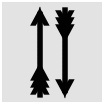
\includegraphics{sl_8_1} \hspace{6em}
    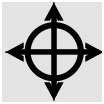
\includegraphics{sl_8_2} \\
    \parbox{11em}{\caption{Воздух}\label{pic-air}} \hspace{1em}
    \parbox{11em}{\caption{Пространство}\label{pic-space}}
  \end{figure}

  Богом пространства на Руси чтят Триглава~-- бога о трех главах, которые, можно
  сказать, символизируют длину ширину и высоту. Кстати, неизменный атрибут
  Триглава~-- огненный меч. Богом морских
  пространств является Переплут~-- в общем, его сущность, понятна из имени,
  этого бога представляют о четырех главах, они символизируют север, юг, запад и
  восток. Бог же ветра~-- это Стрибог со своими младшими братьями~-- Догодой и
  Позвиздом, приятным ветерком и буйным ураганом.

  \chapter*{Заключение}
  \addcontentsline{toc}{chapter}{Заключение}

  Многие языческие символы можно встретить и в настоящее время. Но не каждый
  знает истинное значение того или иного символа. В результате такого незнания
  люди коверкают, неправильно интерпретируют смысл вложенный предками в знаки их
  культуры и обычаев, их религии и повседневной жизни.

  \pagebreak

  \renewcommand{\bibname}{Список литературы}
  \begin{thebibliography}{9}
    \addcontentsline{toc}{chapter}{Список литературы}
    \bibitem{1} Даркевич,~В.~П. Символы небесных светил в орнаменте Древней
      Руси~/ В.~П.~Даркевич.~// Советская археология.~-- 1960.~-- вып.~4.
    \bibitem{2} Рыбаков,~Б.~А. Язычество древних славян~/ Б.~А.~Рыбаков~--
      М.:~Наука.~-- 1981.~-- 608~с.
    \bibitem{3} Аничков,~Е.~В. Язычество и Древняя Русь~/ Е.~В.~Аничков~--
      М.:~Индрик.~-- 2003.~-- 440~с.
    \bibitem{4} Маковский,~М.~М. Сравнительный словарь мифологической символики
      в индоевропейских языках: Образ мира и миры образов~/ М.~М.~Маковский~--
      М.:~Гуманитарный издательский центр ВЛАДОС.~-- 1996.~-- 416~с.
    \bibitem{5} Топоров,~В.~Н. Изобразительное искусство и мифология~/
      В.~Н.~Топоров.~// Мировое дерево. Универсальные знаковые комплексы.
      Т.~2.~-- М.:~Рукописные памятники Древней Руси.~-- 2010.~-- С.~352--388.
    \bibitem{6} Нидерле,~Л. Славянские древности~/ Л.~Нидерле~--
      М.:~Алетейя.~-- 2001.~-- 592~с.
\end{thebibliography}

\end{document}
